\section{引论}

\begin{frame}[fragile]{CH1 引论}
  \begin{easylist} \easyitem
    & 引言
    & 操作系统的目标和作用
    & 操作系统的发展过程(历史)
    & 操作系统的基本特征
    & 操作系统的主要功能
    & 操作系统的结构设计
  \end{easylist}
\end{frame}


\begin{frame}[fragile]{计算机的心智}
  \begin{easylist} \easyitem
    & 玩过游戏吗?程序在计算机上运行的全景是什么样子?

    & 人有心智吗?计算机呢?

    & The Matrix is a computer generated dream world. (43'28'')

    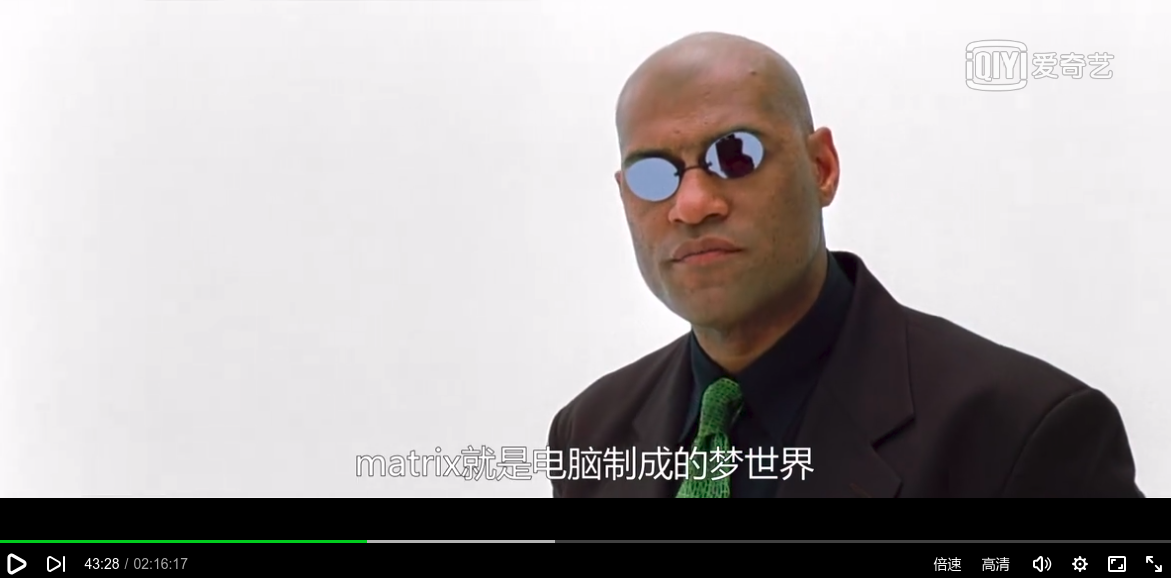
\includegraphics[width=0.8\textwidth]{figure/matrix.png}
    
    && \scriptsize The Matrix itself is a computer program that we (the humans)
    "live" in. It was built by the robots of the future in the great war between
    the humans and robots. The robots designed the matrix so that we would think
    that everything with the world is all right.
  \end{easylist}
\end{frame}


\begin{frame}[fragile]{人造学科的特点}
  \begin{easylist} \easyitem
    & 不精确、具有相对性,没有对错
    & 从对人类活动的观察导出:栈、队列
    & 依赖于人的主观判断力:主观能动性
    & 通常符合人的直觉:如同步机制类似于人的恋爱过程
  \end{easylist}
\end{frame}


\begin{frame}[fragile]{计算机系统组成}
  \begin{easylist} \easyitem
    & 硬件:
    && 计算机物理装置本身(处理器、内存等)
    & 软件:
    && 相对硬件而言,与数据处理系统的操作有关的计算机程序、规则以及相关的文档资料的总称。(简单的说是计算机执行的程序。)包括系统软件和应用软件等。
    & 总线结构:
    && 通过总线连接CPU、内存、键盘、硬盘。。
  \end{easylist}
\end{frame}



\begin{frame}[fragile]{软件分类}
  \begin{easylist} \easyitem
    & 系统软件: 使用和管理计算机
    && {\color{red}操作系统}
    && 数据库管理系统
    && 语言处理程序
    && $\cdots$
    & 应用软件: 解决各种实际问题
    && 通用应用软件,如文字处理软件、电子表格软件等
    && 定制的应用软件
    & 介于二者之间的中间件
    && Web中间件:HTTPD, Nginx, Lighttpd; Tomcat, Jetty,Resin
    && 消息中间件:Kafka, ActiveMQ ...
    && 各种业务中间件 ...
  \end{easylist}
\end{frame}

\begin{frame}[fragile, plain]{~}
  \begin{center}
    桌面OS:
    
    
\includegraphics[width=0.8\textwidth]{figure/mac-win-linux.png}

    手机、平板等移动设备OS:
    
    
\includegraphics[width=0.6\textwidth]{figure/apple_quarreling_with_android.jpg}    
  \end{center}
\end{frame}

\begin{frame}[fragile]{Windows Family}
  \begin{center}
    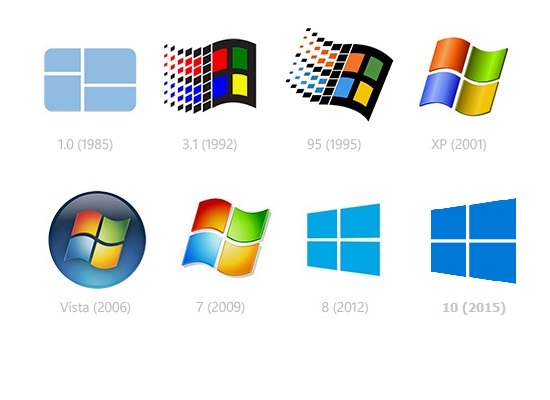
\includegraphics[width=0.8\textwidth]{figure/windows-history.jpg}
  \end{center}
\end{frame}

\begin{frame}[fragile]{操作系统}
  \begin{easylist} \easyitem
    & Microsoft(微软)
    && 最重要的软件产品(立家之本)
    && 操作系统(Windows)
    & Apple
    && iOS
    & 主要IT软件厂商多有涉足:
    && IBM, Oracle(Sun\footnote{2009年4月20日甲骨文以74亿美元现金收购Sun微系统公司。}), Redhat\footnote{2018年10月29日早晨,IBM宣布以340亿美元的价格收购Red Hat。},Google, Alibaba, 鸿蒙…
    && AIX, Solaris, Android, FreeBSD, SuSE, Ubuntu…
    & Virtual Machine
    && VMwareWorkstation
    && VirtualBox
  \end{easylist}
\end{frame}


\begin{frame}[fragile]{为什么学习操作系统}
  \begin{easylist} \easyitem
    & 操作系统已经深入到我们生活中的方方面面
    && 存在人们意识不到的大量“操作系统”%(如:嵌入式系统-家电、手机)
    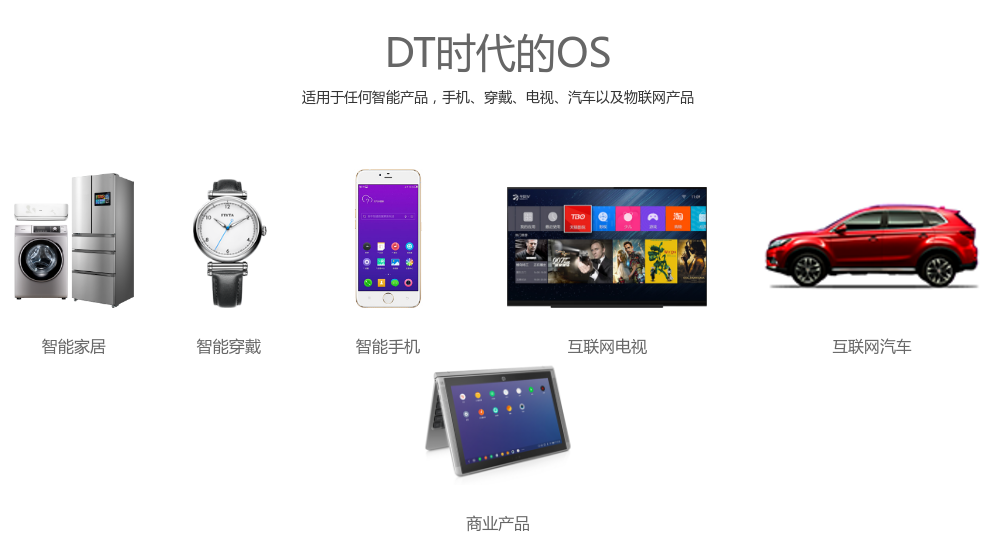
\includegraphics[width=0.5\textwidth]{figure/yunos.png}
    & 优秀程序员必不可少的基础知识
    && 加深对操作系统的理解,有利于深入编程;用户为了开发应用程序必须与操作系统打交道
    && 借鉴操作系统的设计思想和算法(插件、微内核)
    && 设计操作系统或者修改现有的系统
    && Switch 和 If,哪个效率更高?
  \end{easylist}
\end{frame}

\begin{frame}[fragile]{为什么学习操作系统(2)}
  \begin{easylist}
    & 理解操作系统原理是掌握某些知识的必备基础,如大数据、云计算、分布式、WebService...
    & 操作系统中所用的许多概念和技巧可以推广应用到其他领域(如先来先服务、短作业
    优先…)
    & 可以提高情商 :)
	  \begin{tcolorbox}[colback=green!5,colframe=green!50,title=What's the meaning?]
		me@my-desktop:\~ \$ chmod 700 myfate \\
		  Permission denied 
	  \end{tcolorbox}

%    \begin{block}{What's the meaning?}
%      me\@me-desktop:~\$ chmod 700 myfate \\
%      Permission denied 
%    \end{block}
  \end{easylist}
\end{frame}


\begin{frame}[fragile, plain]
%  \frametitle{如何选用操作系统}
  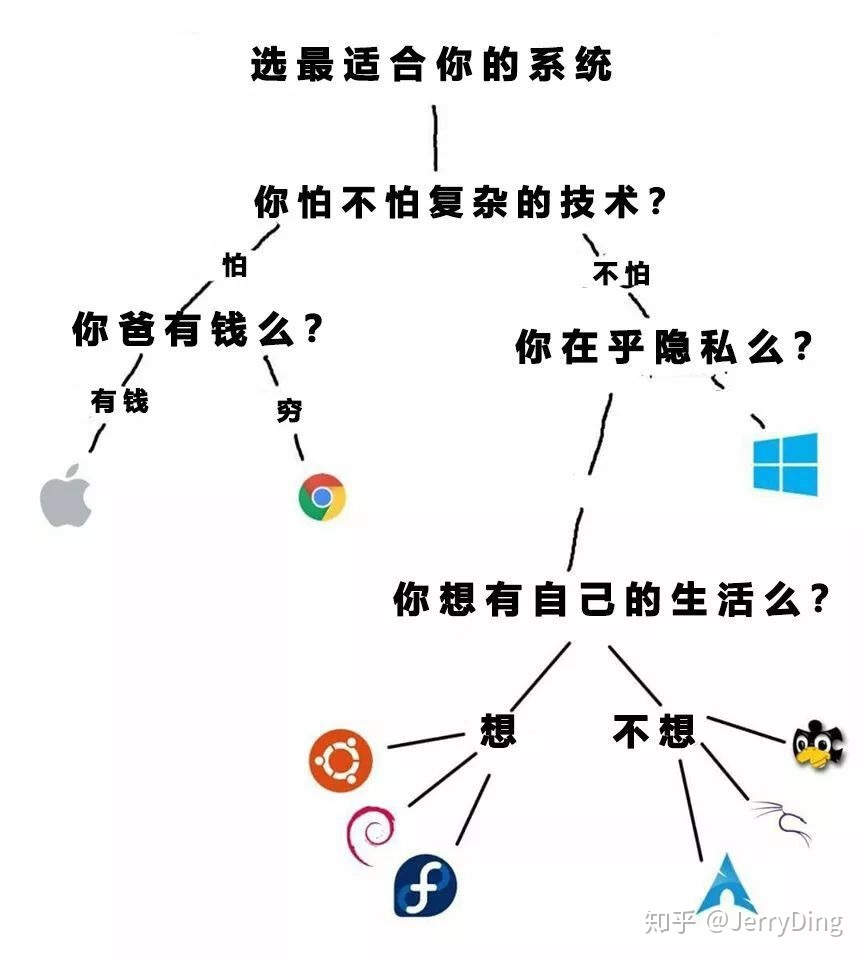
\includegraphics[width=0.7\textwidth]{figure/best_os.jpg}
  From: https://www.zhihu.com/question/267941005/answer/564103434
\end{frame}


\begin{frame}[fragile]{操作系统涉及的领域}
  \begin{easylist} \easyitem
    & 计算机体系结构/硬件
    & 软件设计
    & 程序设计语言
    & 数据结构
    & 算法
    & 网络
  \end{easylist}
  学习核心技术并能在其他地方应用

  操作系统是目前最复杂的软件系统
\end{frame}


\begin{frame}[fragile]{如何学好本课程}
  \begin{easylist} \easyitem
    & 理论学习
    & 实验、实习
    & 源代码分析、参与(Linux)
    & 多读相关书籍
  \end{easylist}
\end{frame}


\begin{frame}[fragile]{参考书目}
  \begin{easylist} \easyitem
    & 汤小丹, 汤子瀛等. 《计算机操作系统(第4版)》, 西安电子科技大学 
    && 附带学习指导与题解
    & 张尧学等.《计算机操作系统教程(第4版)》,清华大学出版社
    & 操作系统精髓与设计原理
    & Silberschatz,《操作系统概念》(中、英文)第9版,高等教育出版社
  \end{easylist}
\end{frame}


\begin{frame}[fragile]{推荐阅读}
  \begin{easylist} \easyitem
    & 深入理解计算机系统,机械工业出版社
    & 操作系统之哲学原理
    & 鸟哥的Linux私房菜
    & 现代操作系统(原书第4版),机械工业出版社
  \end{easylist}
\end{frame}


\begin{frame}[fragile]{问题交流}
  \begin{easylist} \easyitem 
    & 问题交流:
    && 课堂交流(可随时留言)
    && 微信群
    && 助教:梁艺耀
  \end{easylist}
\end{frame}


\begin{frame}[fragile]{讨论时间}
  \begin{easylist} \easyitem
    & 如果让你设计一个操作系统:
    && 你想到的功能都有哪些?请列举主要方面。
    && 你觉得未来的操作系统会往哪些方面发展/你最期待的功能是什么?
    && 一刻钟后发到留言部分
    & 调查有哪些操作系统,把LOGO和名称发到群里面。
  \end{easylist}
\end{frame}

\subsection{1.1 操作系统的目标和作用}
\begin{frame}[fragile]{1.1 操作系统的目标和作用}
  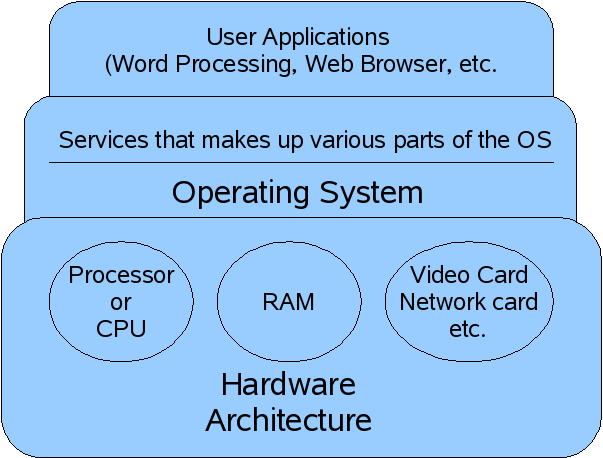
\includegraphics[width=0.8\textwidth]{figure/intro_os_diagram.png}
\end{frame}


\begin{frame}[fragile]{1.1.1 操作系统的目标}
  \begin{easylist} \easyitem
    & 方便性
    & 有效性
    & 可扩展性
    & 开放性
  \end{easylist}
\end{frame}


\begin{frame}[fragile]{1.1.2 操作系统的作用}
  \begin{easylist} \easyitem
    & (1) OS作为用户与计算机硬件系统之间的接口
    && 语音、视频接口
    && 图形用户接口
    && 命令接口
    && 系统调用接口
  \end{easylist}
  \begin{center}
    \begin{tikzpicture}[box/.style={draw,minimum height=0.7cm}]
      \draw[] node[box, minimum width=8cm] (hardware) {计算机硬件}
      node[box, minimum width=7cm, fill=red!10, align=center, above=0 of hardware] (os) {操作系统}
      node[box, above=0 of os, minimum width=2cm, xshift=-2cm] (sc) {系统调用}
      node[box, right=0 of sc] (cmd) {命令}
      node[box, right=0 of cmd] (gui) {窗口} 
      node[box, right=0 of gui] (voice) {语音、视频...} ;

      \draw[] node[box, above=0 of sc, minimum width=2cm] (app) {应用程序} ;
      \draw[] node[box, above=0 of app, minimum width=6cm, xshift=2cm] (user) {用户};
      \draw[latex-latex, very thick] ++(user.south) ++(-0,0)--++(0,-0.7);
      \draw[latex-latex, very thick] ++(user.south) ++(1.5,0)--++(0,-0.7);
    \end{tikzpicture}
  \end{center}
\end{frame}

\begin{frame}[fragile]
  \frametitle{iPhone X ditches Touch ID for Face ID\footnote{\url{https://venturebeat.com/2017/09/12/iphone-x-ditches-touch-id-for-face-id/}}}
  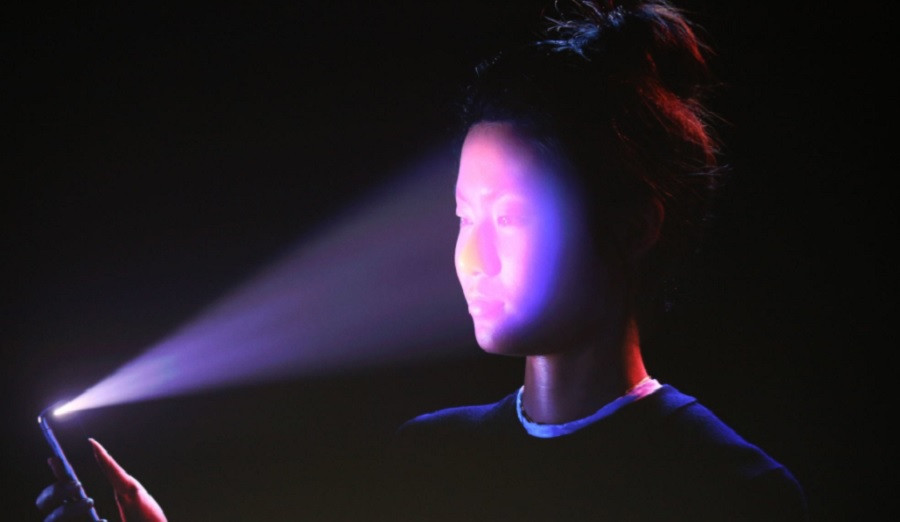
\includegraphics[width=0.85\textwidth]{figure/intro_face_id.jpg} 
\end{frame}


\begin{frame}[fragile]{1.1.2 操作系统的作用}
  \begin{easylist} \easyitem
    & (2) OS作为计算机系统资源的管理者
    && 处理机管理,用于分配和控制处理机;
    && 存储器管理,主要负责内存的分配与回收;
    && I/O设备管理,负责I/O设备的分配与操纵;
    && 文件管理,负责文件的存取、共享和保护。
  \end{easylist}
\end{frame}


\begin{frame}[fragile]{1.1.2 操作系统的作用}
  \begin{easylist} \easyitem
    & (3) OS用作扩充机器
    && 通常把覆盖了软件的机器称为扩充机器(Extended Machine)或虚机器(Virtual Machine)
  \end{easylist}
\end{frame}


\begin{frame}[fragile]{操作系统:魔幻家与管理者}
  \begin{easylist} \easyitem
    & 魔幻家
    && 差的东西变好:不用直接与硬件指令打交道,如磁盘的控制管理
    && 少得东西变多:虚拟内存
    && 无中生有:如逻辑盘, WPS网盘
    & 管理者
    && CPU管理
    && 内存管理
    && 外存管理
    && IO管理
  \end{easylist}
\end{frame}


\begin{frame}[fragile]{1.1.3 推动OS发展的主要动力}
  \begin{easylist} \easyitem
    & 不断提高计算机资源利用率
    & 方便用户
    & 器件的不断更新换代
    & 计算机体系结构的不断发展
    & 操作系统的攻击与防范
    && 病毒和木马在一定程度上促进了操作系统的发展
    & 其他:
    && 价格、可靠性等
  \end{easylist}
\end{frame}



\begin{frame}[fragile]{硬件成本的不断下降举例}
  \begin{easylist} \easyitem
    & IBM制造的第一张硬盘RAMAC 350(1956/9/4),容量只有5M,重达一吨,需要一家飞机来运。
    & 硬件成本的下降使得操作系统可以变得更为复杂,使操作系统从最初的几百行代码、
    几千行代码变为4000万行代码的复杂系统(Windows XP),Linux 2.6.7内核超过1000万行
  \end{easylist}
  \centering
  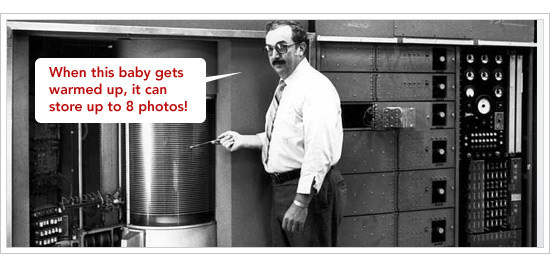
\includegraphics[width=0.7\textwidth]{figure/intro_first_disk2.jpg}
  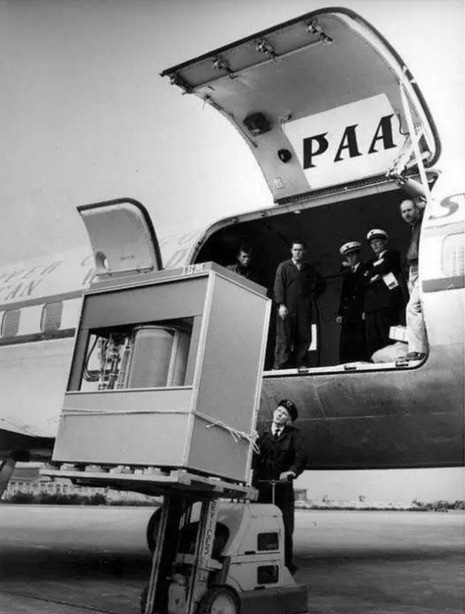
\includegraphics[width=0.25\textwidth]{figure/intro_first_disk1.jpg}
\end{frame}

\subsection{1.2 操作系统的发展历程}
\begin{frame}[fragile]{1.2 操作系统的发展历程}
  \begin{easylist} \easyitem
    & 状态机操作系统(1940年以前)
    & 单一操作员单一控制终端(20世纪40年代)
    & 批处理操作系统
    && UMES
    & 多道批处理操作系统
    && OS/360
    & 分时系统
    && Unix
    & 实时操作系统
    & 现代操作系统
  \end{easylist}
\end{frame}


\begin{frame}[fragile]{1.2.1 第一代计算机(手工操作阶段)}
  \begin{easylist} \easyitem
    & 1. 完全人工操作方式
    && 缺点:
    &&& 用户独占全机
    &&& CPU等待人工操作
    & 2. 脱机输入/输出(Off-Line I/O)方式
  \end{easylist}
\end{frame}


\begin{frame}[fragile]{脱机输入/输出示例}
  \begin{center}
    \begin{tikzpicture}[box/.style={draw, align=center,minimum height=1cm,minimum width=2.cm, fill=yellow!10},
      database/.style={ cylinder, cylinder uses custom fill,
        fill=green!2, align=center, shape border rotate=90, aspect=0.15,
        inner sep=0.2cm, minimum width=2.cm, minimum height=1cm, draw},
      multidocument/.style={
        shape=tape,
        draw,
        fill=gray!5,
        tape bend top=none,
        minimum height=1cm,
        minimum width=2.cm,},
      link/.style={draw, thick,-{Latex[scale=1.2]}},
      scale=0.6]
      \draw node[multidocument] (input) {输入设备}
      node[box,right=of input] (w1) {外围机}
      node[database,right=of w1](disk1) {磁盘} ;
      \draw[link] (input)--(w1);
      \draw[link] (w1)--(disk1);

      \draw node[database, below=of input, very thick, draw=red!60] (disk2) {磁盘}
      node[box,right=of disk2, very thick, draw=red!60] (main) {主机}
      node[database,right=of main, very thick, draw=red!60] (disk3) {磁盘} ;
      \draw[link] (disk2)--(main);
      \draw[link] (main)--(disk3);

      \draw node[database, below=of disk2] (disk4) {磁盘}
      node[box,right=of disk4] (w2) {外围机}
      node[multidocument,right=of w2] (output) {输出设备} ;
      \draw[link] (disk4)--(w2);
      \draw[link] (w2)--(output);
    \end{tikzpicture}
  \end{center}
  \begin{easylist} \easyitem
    & 优点:
    && 减少了CPU的空闲时间。
    && 提高了I/O速度。
  \end{easylist}
\end{frame}




\begin{frame}[fragile]{1.2.2 单道批处理系统}
  \begin{easylist} \easyitem
    & 单道批处理系统(Simple Batch Processing System)的处理过程
    & 单道程序运行情况
    && 特征:(1)自动性; (2)顺序性; (3) 单道性
  \end{easylist}
  \begin{center}
\scalebox{0.77}{
    \begin{tikzpicture}[tip/.style={ minimum height=1cm,minimum width=2.cm}]
      \draw node[tip] (user) {用户程序} node[tip, below=0.2cm of user] (jiandu) {监督程序}  node[tip, below=0.2cm of jiandu] (io) {I/O操作};

      \draw node[tip, right=of user, ] (jisuan) {计算}
      node[tip,right=0 of jisuan] (input) {请求输入}
      node[tip, right=0 of input] (b14){}
      node[tip, right=0 of b14] (b15){}
      node[tip, right=0 of b15, ] (b16) {继续计算} ;

      \draw node[tip, right=of jiandu] (b22){}
      node[tip, right=0 of b22] (b23) {启动I/O}
      node[tip, right=0 of b23] (b24) {}
      node[tip, right=0 of b24] (b25) {I/O完成};

      \draw node[tip, right=of io] (b32){}
      node[tip, right=0 of b32] (b33) {}
      node[tip, right=0 of b33] (b34) {}
      node[tip, right=0 of b34] (b35) {结束中断};

      \draw[draw=blue!60,line width=2pt] (2, -0.5)--(4,-0.5) (4,-1.7)--(6,-1.7) (6,-2.9)--(8,-2.9)  (8,-1.7)--(10,-1.7) (10,-0.5)--(12,-0.5);
      \draw[dashed] (4,-0.5)--(4,-1.6) (6,-1.7)--(6, -2.9) (8, -1.7)--(8, -2.9) (10,-0.5)--(10,-1.6);
    \end{tikzpicture}
}
  \end{center}
\end{frame}


\begin{frame}[fragile]{单道批处理系统示例}
  \begin{center}
    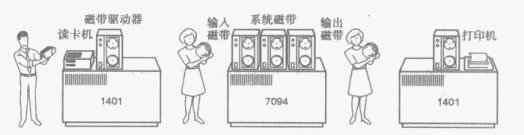
\includegraphics[width=0.9\textwidth]{figure/intro-batch_os.jpg}
  \end{center}
\end{frame}


\begin{frame}[fragile]{密歇根执行系统UMES}
  \begin{easylist} \easyitem
    & MAD/UMES
    && R.M.Graham, Bruce Arden, Bernard Galler
    && 密歇根算法译码器/密歇根大学执行系统
  \end{easylist}

  \begin{columns}[onlytextwidth]
    \begin{column}{0.5\textwidth}
      \centering
      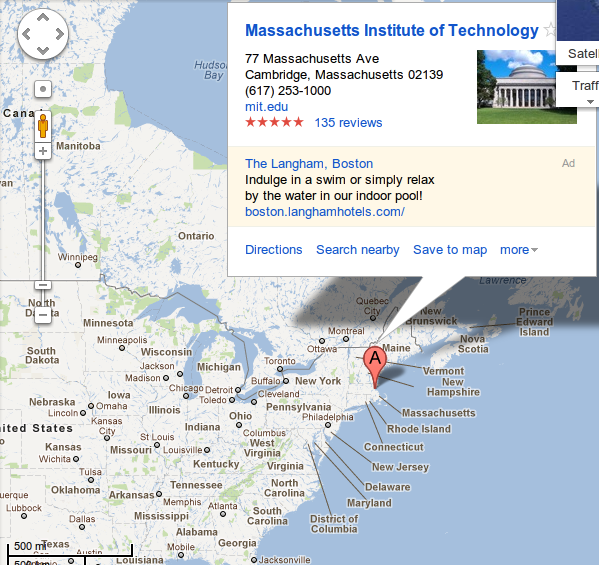
\includegraphics[width=0.9\textwidth]{figure/intro-mit_location.jpg}
    \end{column}
    \begin{column}{0.5\textwidth}
      \centering
      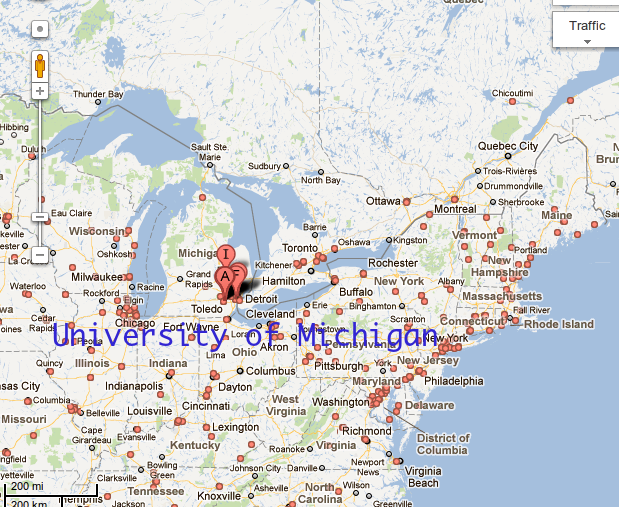
\includegraphics[width=0.9\textwidth]{figure/intro-michigan_location.jpg}
    \end{column}
  \end{columns}
\end{frame}



\begin{frame}[fragile]{1.2.3 多道批处理系统}
  \begin{easylist} \easyitem
    & 多道批处理系统运行过程示例
  \end{easylist}
  \centering
  \begin{tikzpicture}[tip/.style={ minimum height=1cm,minimum width=2.cm},
    box/.style={draw, minimum height=0.8cm,minimum width=1.5cm},
    line/.style={very thick, draw=blue!50}
    ]

    \draw[] node[tip] (a) {程序A}
    node[tip,below=0.2cm of a] (b) {程序B}
    node[tip,below=0.2cm of b] (c) {程序C}
    node[tip,below=0.2cm of c] (d) {程序D}
    node[tip,below=0.2cm of d] (e) {处理器} ;

    \draw[] node[box, right=0 of a] {运行} node[box, right=7.5cm of a] {运行};
    \draw[line] (0.8,-0.45)--(10.5,-0.45);

    \draw[] node[box, right=3cm of b] {运行} node[box, right=6cm of b] {运行};
    \draw[line] (0.8,-1.65)--(10.5,-1.65);

    \draw[] node[box, right=4.5cm of c] {运行};
    \draw[line] (0.8,-2.85)--(10.5,-2.85);

    \draw[] node[box, right=1.5cm of d] {运行};
    \draw[line] (0.8,-4.1)--(10.5,-4.1);

    \draw[] node[box, right=0 of e] (e2) {运行}
    node[box, right=0 of e2] (e3) {运行}
    node[box, right=0 of e3] (e4) {运行}
    node[box, right=0 of e4] (e5) {运行}
    node[box, right=0 of e5] (e6) {运行}
    node[box, right=0 of e6] (e7) {运行};
    \draw[line, draw=red!60] (0.8,-5.3)--(10.5,-5.3);

    \draw[line, -Latex] (2,-6)--(8,-6) node[right] {时间};
  \end{tikzpicture}
\end{frame}


\begin{frame}[fragile]{多道批处理系统}
  \begin{easylist} \easyitem
    & 特征
    && 多道性
    && 无序性
    && 调度性
  \end{easylist}
\end{frame}


\begin{frame}[fragile]{多道批处理系}
  \begin{easylist} \easyitem
    & 优缺点
    && 资源利用率高
    && 系统吞吐量大
    && 平均周转时间长
    && 无交互能力
  \end{easylist}
\end{frame}


\begin{frame}[fragile]{多道批处理系统}
  \begin{easylist} \easyitem
    & 需要解决的问题
    && 处理机管理问题
    && 内存管理问题
    && I/O设备管理问题
    && 文件管理问题
    && 作业管理问题
  \end{easylist}
\end{frame}


\begin{frame}[fragile]{代表OS}
  \begin{easylist} \easyitem
    & IBM OS/360
    && 运行于IMB System 360、370、4300
    && 引入了内存的分段管理
  \end{easylist}
\end{frame}


\begin{frame}[fragile]{操作系统的定义}
  一组控制和管理计算机硬件和软件资源、合理地对各类作业进行调度、以及方便用户的程序的集合
\end{frame}


\begin{frame}[fragile]{操作系统的定义}
  \begin{easylist} \easyitem
    & 说明
    && 操作系统是软件,是系统软件,是由一整套程序组成。
    && 基本职能:控制和管理系统内各种资源,有效地组织多道程序地运行
    && 提供众多服务,方便用户使用,扩充硬件功能。
    && 操作系统的地位:其他软件的支撑环境
  \end{easylist}
\end{frame}


\begin{frame}[fragile]{1.2.4 分时系统}
  \begin{easylist} \easyitem
    & 1. 分时系统(Time-Sharing System)的产生
    && 用户的需求具体表现在以下几个方面:
    && (1) 人—机交互
    && (2) 共享主机
    && (3) 便于用户上机
  \end{easylist}
\end{frame}


\begin{frame}[fragile]{1.2.4 分时系统}
  \begin{easylist} \easyitem
    & 2. 分时系统实现中的关键问题
    && (1) 及时接收
    && (2) 及时处理
  \end{easylist}
\end{frame}


\begin{frame}[fragile]{1.2.4 分时系统}
  \begin{easylist} \easyitem
    & 3. 分时系统的特征
    && (1)多路性。(宏观:多用户同时工作,共享系统资源;微观:用户作业轮流运行 )
    && (2) 独立性
    && (3) 及时性
    && (4) 交互性
  \end{easylist}
\end{frame}


\begin{frame}[fragile]{代表性OS}
  \begin{easylist} \easyitem
    & Multics、Unix
    && 密歇根的R.M.Graham主持,MIT、DEC、贝尔实验室
    && 贝尔实验室 $\Rightarrow$ 单干 $\Rightarrow$ Unix $\Rightarrow$ 图灵奖
    && MIT $\Rightarrow$ 应用于商用领域的分时系统CTSS
  \end{easylist}
\end{frame}


\begin{frame}[fragile]{1.2.5 实时系统}
  \begin{easylist} \easyitem
    & 1. 应用需求
    && (1) 实时控制
    && (2) 实时信息需求
  \end{easylist}
\end{frame}

\begin{frame}[fragile]{1.2.5 实时系统}
  \begin{easylist} \easyitem
    & 2. 定义
    && 实时:
    &&& 指对随机发生的外部事件做出及时的相应并对其进行处理。(所谓事件是指来自与计算机系统相连接的设备所提出的服务要求和采集数据)
    && 实时系统:
    &&& 指系统能及时(或即时)响应外部事件的请求,在规定的时间内完成对该事件的处理,并控制所有实时任务协调一致地运行
  \end{easylist}
\end{frame}

\begin{frame}[fragile]{1.2.5 实时系统}
  \begin{easylist} \easyitem
    & 3. 实时任务
    && 1) 按任务执行时是否呈现周期性来划分
    &&& (1) 周期性实时任务
    &&& (2) 非周期性实时任务
    && 2) 根据对截止时间的要求来划分
    &&& (1) 硬实时任务(hard real-time task)
    &&& (2) 软实时任务(Soft real-time task)
  \end{easylist}
\end{frame}

\begin{frame}[fragile]{1.2.5 实时系统}
  \begin{easylist} \easyitem
    & 4.实时系统与分时系统特征的比较
    && (1) 多路性
    && (2) 独立性
    && (3) 及时性
    && (4) 交互性
    && (5) 可靠性
  \end{easylist}
\end{frame}


\begin{frame}[fragile]{现代操作系统}
  \begin{easylist} \easyitem
    & 受益于80年代后计算机工业的快速发展
    & 价格下降使得个人有能力独享计算机
    & 个人独享使得分时系统的某些功能不再需要,似乎又回到了早期的SOSC阶段的标准函数库方式
    & 分时的需求
    & 网络的需求
  \end{easylist}
\end{frame}


\begin{frame}[fragile]
  \frametitle{云操作系统}
  云计算是一种新兴的IT资源的交付和使用方式,通过网络以按需、易于扩展的方式获得所
  需资源。提供资源的网络称为“云”。

  云操作系统COS就是对云进行管理的操作系统

  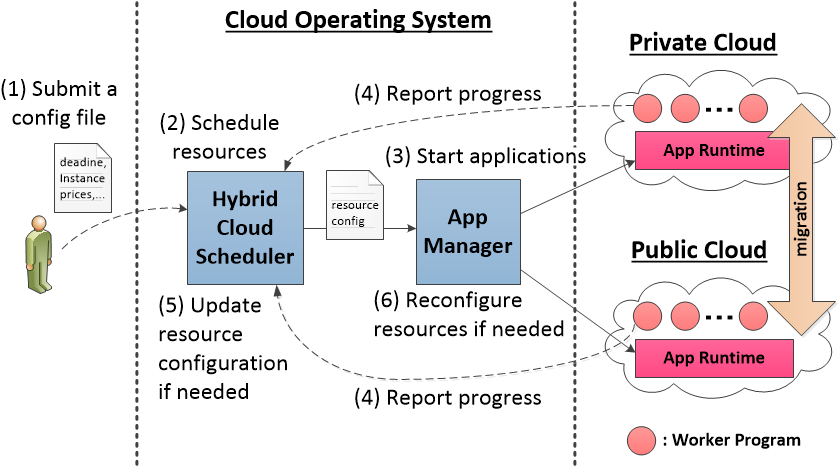
\includegraphics[width=0.8\textwidth]{figure/cos/arch.png}
\end{frame}


\begin{frame}[fragile]
  \frametitle{IaaS, PaaS, SaaS}
  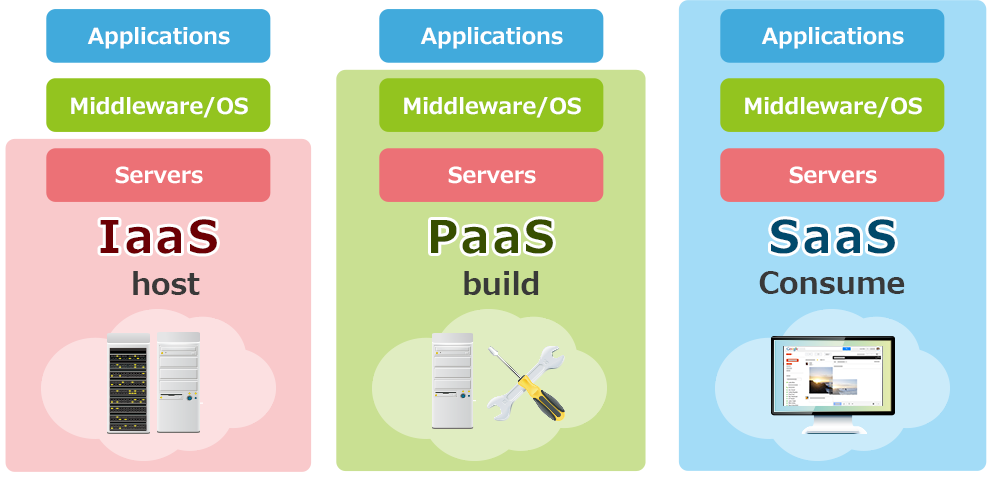
\includegraphics[width=0.8\textwidth]{figure/cos/iaas.png}
\end{frame}

\begin{frame}[fragile]
  \frametitle{IaaS, PaaS, SaaS}
  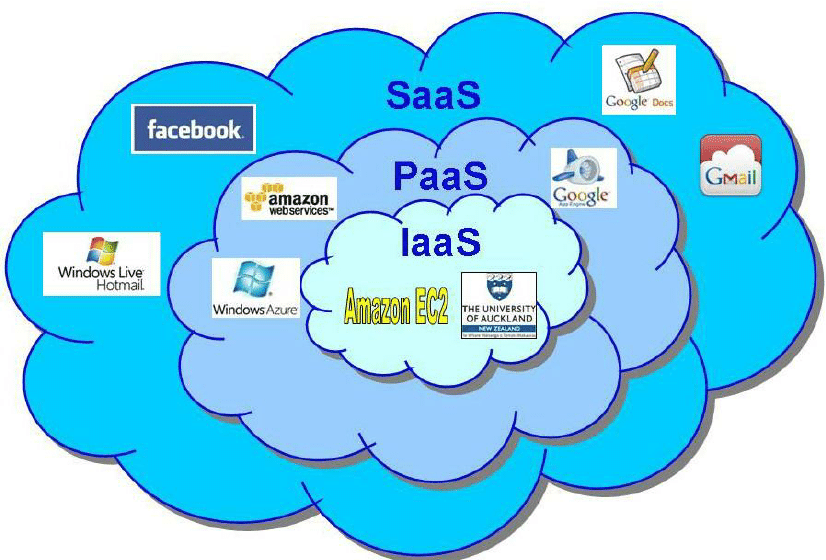
\includegraphics[width=0.8\textwidth]{figure/cos/iaas2.png}
\end{frame}


\begin{frame}[fragile]{操作系统的演变}
\begin{center}
  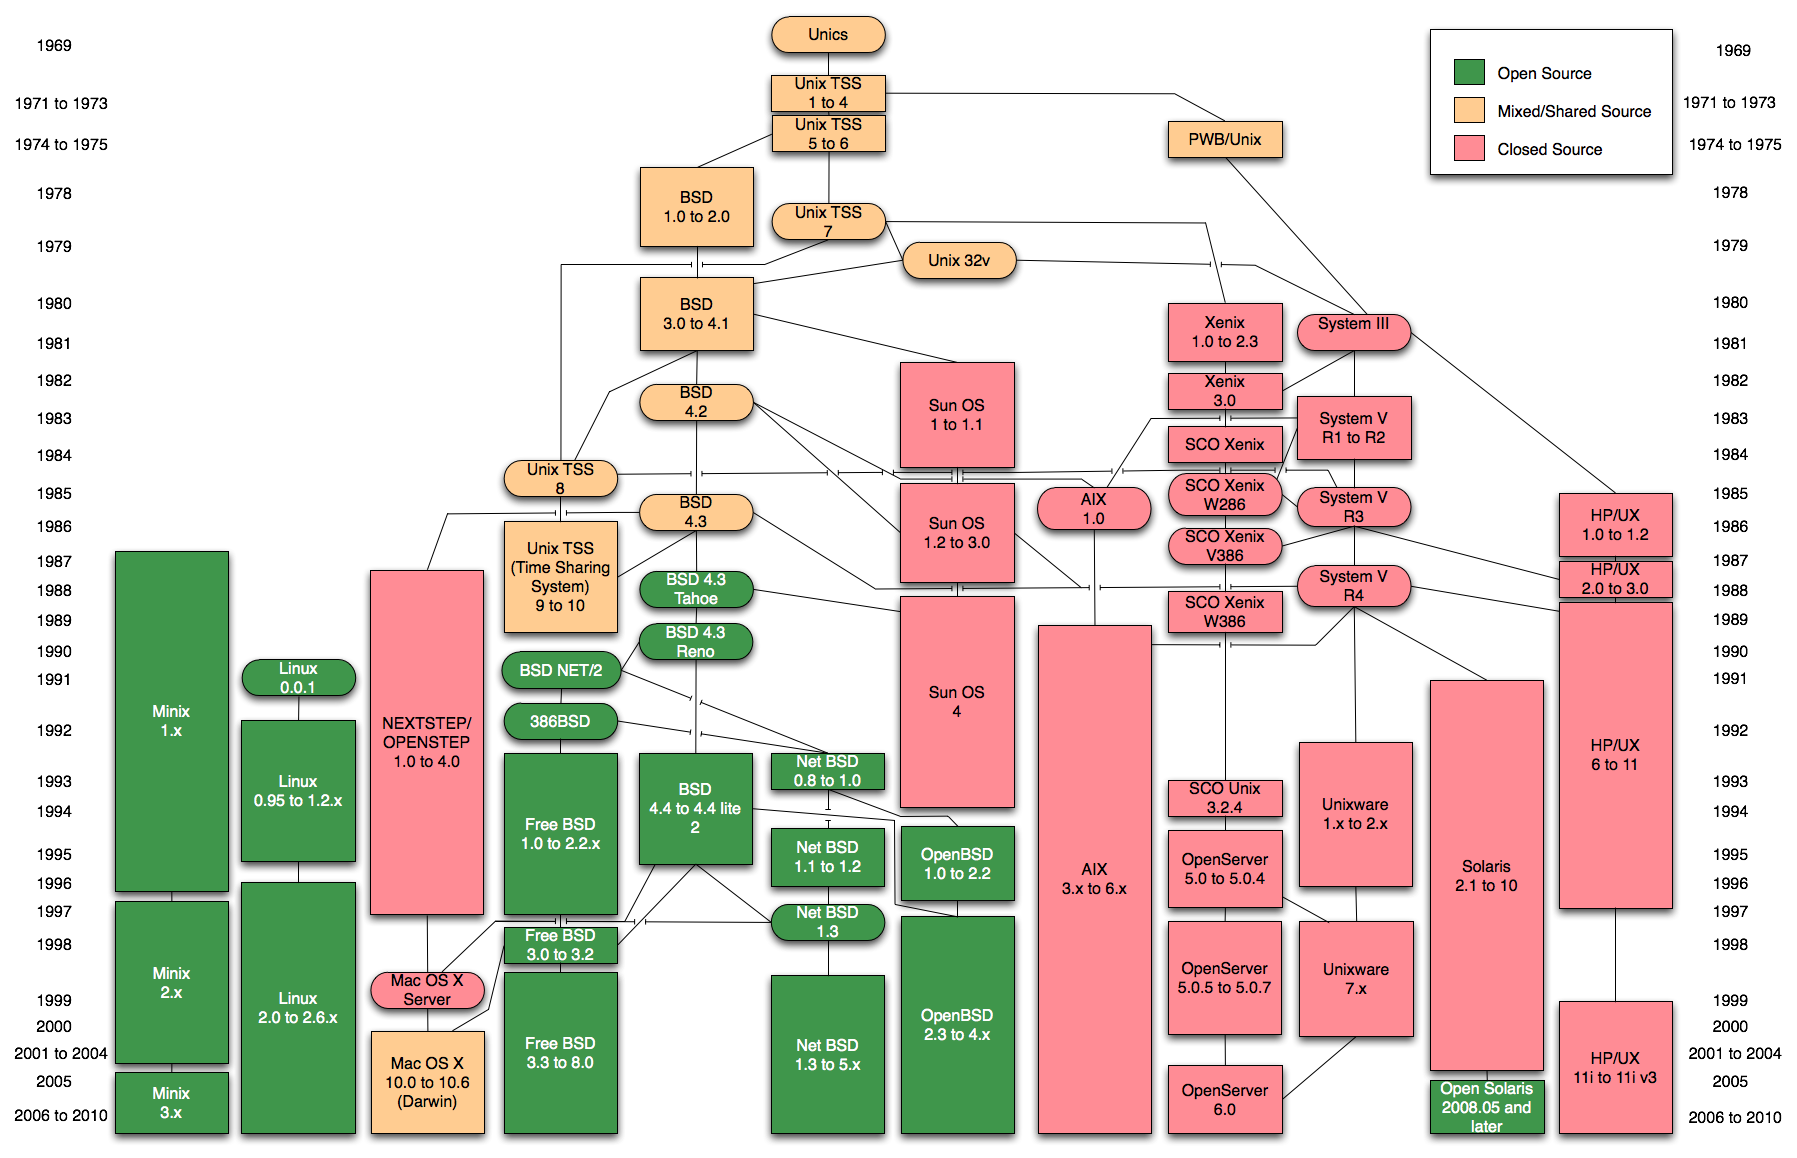
\includegraphics[width=0.9\textwidth]{figure/intro-unix_history-simple.png}
\end{center}
\end{frame}


\begin{frame}[fragile]{补充:计算机发展史}
  \begin{easylist}
    & 微型电脑就是一部缩小了的小型机 \footnote{https://www.zhihu.com/question/49073893}
  \end{easylist}

  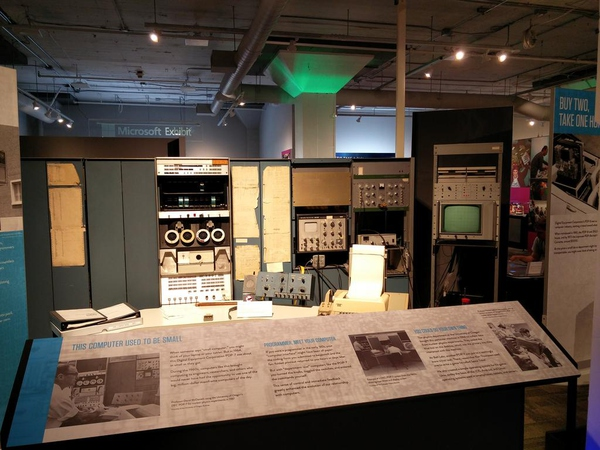
\includegraphics[width=0.9\textwidth]{figure/intro-minicomputer.jpg}
\end{frame}

\begin{frame}[fragile]{控制台tty}
  \begin{easylist}
    & 在类Unix里,键盘显示器,都是虚拟的teletypewriter
    & 真正的teletypewriter长这样
  \end{easylist}
  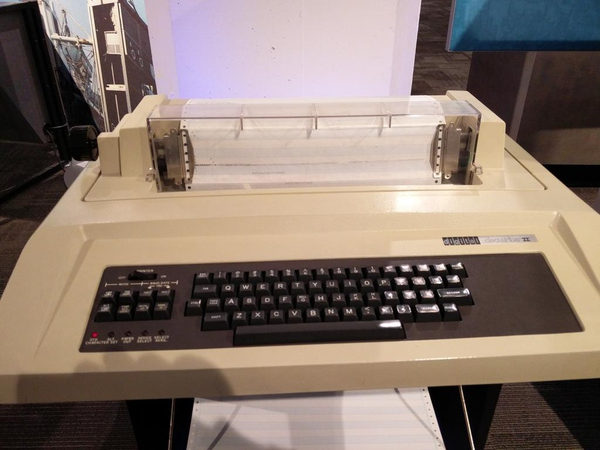
\includegraphics[width=0.9\textwidth]{figure/intro-tty.jpg}
\end{frame}

\begin{frame}[fragile]{tar命令解压缩}
  \begin{easylist}
    & 为什么解压缩往往会用到tar -zxvf?这个tar命令究竟是什么?
    & 实物版的tar长这样,叫Tape Archive
  \end{easylist}
  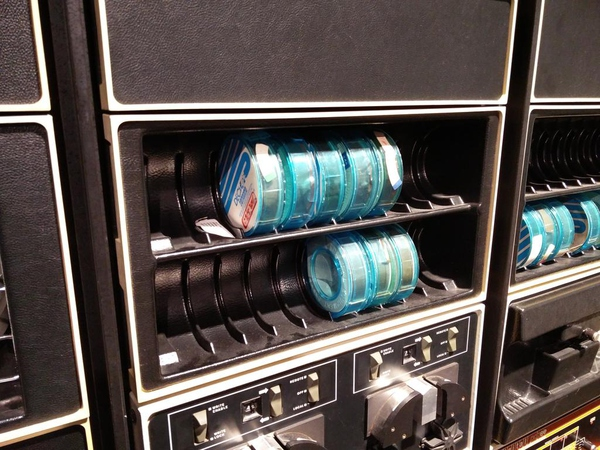
\includegraphics[width=0.9\textwidth]{figure/intro-tar.jpg}
\end{frame}

\begin{frame}[fragile]{为什么硬盘要mount/umount}
  \begin{easylist}
    & 硬盘都是固定在电脑里的,mount管什么用?这货叫DEC Pack,就是数据库图标里的那个圆柱,要让这圆柱(硬盘)工作起来,先得把它放进硬盘驱动器,这个驱动器就叫/dev/hda(也可能是hdb,看一共有几个Hard Drive)。
  \end{easylist}
  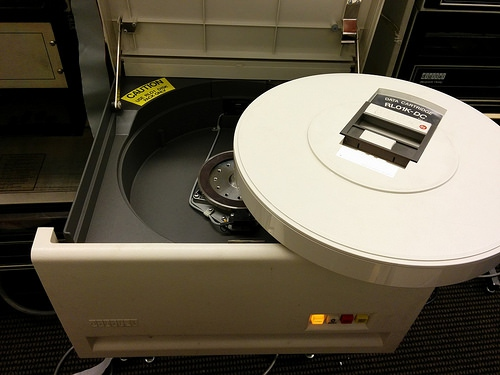
\includegraphics[width=0.9\textwidth]{figure/intro-mount.jpg}
\end{frame}

\begin{frame}[fragile]{结论}
  \begin{easylist}
    & 计算机的原理都是一样的,只是尺寸变小后这些部分{\color{red}看起来}像是一体
    的。
    & 课外阅读:带你逛西雅图活电脑博物馆
  \end{easylist}
\end{frame}

\begin{frame}[fragile]{操作系统的“差不多”精神}
  \begin{easylist} \easyitem
    & 与数学相比软件学科具有“差不多”特点
    && 数学家与软件专家的故事
    && 差不多:如“算法复杂度”
  \end{easylist}
\end{frame}

\subsection{1.3 操作系统的四个基本特征}
\begin{frame}[fragile]{1.3 操作系统的四个基本特征}
  \begin{easylist} \easyitem
    & 并发(Concurrence)
    & 共享(Sharing)
    & 虚拟(Virtual)
    & 异步性(Asynchronism)
  \end{easylist}
\end{frame}


\begin{frame}[fragile]{1.3.1 并发}
  \begin{easylist} \easyitem
    & 并行性:
    && 是指两个或多个事件在同一时刻发生;
    & 并发性:
    && 是指两个或多个事件在同一时间间隔内发生。
  \end{easylist}
  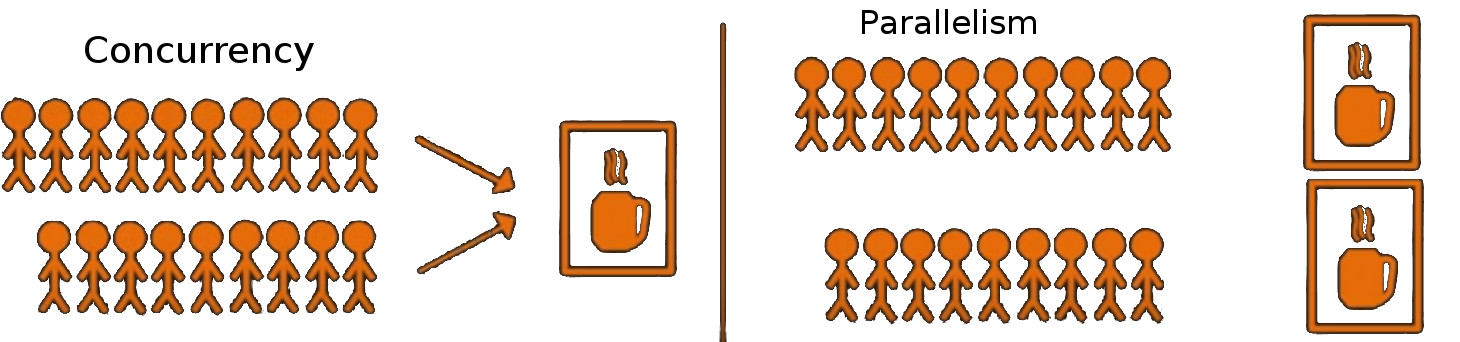
\includegraphics[width=0.9\textwidth]{figure/parallel.jpg}
\end{frame}


\begin{frame}[fragile]{1.3.2 共享}
  \begin{easylist} \easyitem
    & 互斥共享方式
    & 同时访问方式

    & 例如:
    && 三个程序在同一时间间隔内访问磁盘
    && 多个程序在同一时间间隔内要求打印文本
  \end{easylist}
\end{frame}


\begin{frame}[fragile]{1.3.3 虚拟}
  \begin{easylist} \easyitem
    & “虚拟”:是指通过某种技术把一个物理实体变为若干个逻辑上的对应物。相应地,用于实现虚拟的技术,称为虚拟技术。
  \end{easylist}
\end{frame}


\begin{frame}[fragile]{1.3.4 异步性}
  \begin{easylist} \easyitem
    & 假设能同时双击两个大小相同的Word文档,你能断定哪一个先打开吗?
    & 进程是以人们不可预知的速度向前推进,此即进程的异步性
  \end{easylist}
\end{frame}


\subsection{1.4 操作系统的主要功能}
\begin{frame}[fragile]{1.4 操作系统的主要功能}
  \begin{easylist} \easyitem
    & 1.4.1 处理机管理
    && (1) 进程控制
    && (2) 进程同步
    &&& ① 进程互斥方式:诸进程(线程)在对临界资源进行访问时,应采用互斥方式;
    &&& ② 进程同步方式:指在相互合作去完成共同任务的诸进程(线程)间,由同步机构对它们的执行次序加以协调。
    && (3) 进程通信
    && (4) 调度
  \end{easylist}
\end{frame}


\begin{frame}[fragile]{1.4.2 存储器管理}
  \begin{easylist} \easyitem
    & 1. 内存分配
    && 分配方式:
    &&& 静态分配方式、动态分配方式
    && 在内存分配的机制中应具有这样的结构和功能:
    &&& ① 内存分配数据结构
    &&& ② 内存分配功能
    &&& ③ 内存回收功能
  \end{easylist}
\end{frame}


\begin{frame}[fragile]{1.4.2 存储器管理}
  \begin{easylist} \easyitem
    & 2. 内存保护
    && 确保每道用户程序都只在自己的内存空间内运行,彼此互不干扰。
  \end{easylist}
\end{frame}


\begin{frame}[fragile]{1.4.2 存储器管理}
  \begin{easylist} \easyitem
    & 3. 地址映射
    && “逻辑地址”或“相对地址”。
    && “物理地址”
  \end{easylist}
\end{frame}


\begin{frame}[fragile]{1.4.2 存储器管理}
  \begin{easylist} \easyitem
    & 4. 内存扩充
    && 借助于虚拟存储技术,从逻辑上去扩充内存容量
    && 为了能在逻辑上扩充内存,系统必须具有内存扩充机制, 用于实现下述各功能:
    &&&  (1) 请求调入功能
    &&& (2) 置换功能
  \end{easylist}
\end{frame}


\begin{frame}[fragile]{1.4.3 设备管理}
  \begin{easylist} \easyitem
    & 缓冲管理
    & 设备分配和设备处理
    & 虚拟设备等功能。
  \end{easylist}
\end{frame}


\begin{frame}[fragile]{1.4.4 文件管理}
  \begin{easylist} \easyitem
    & 1. 文件存储空间的管理
    && 相应的数据结构,存储空间的分配和回收功能。
    && 通常是采用离散分配方式,以减少外存零头,并以盘块为基本分配单位。盘块的大小通常为512 B\~8 KB。
    & 2. 目录管理
    & 3. 文件的读写管理与保护
  \end{easylist}
\end{frame}


\begin{frame}[fragile]{1.4.5 用户接口}
  \begin{easylist} \easyitem
    & 1. 系统调用
    & 2. 壳(Shell)
    && 命令,如Linux Shell,可运行多个
    && 图形,如Windows Explorer,保持一个实例
    \vspace{1cm}
    & 示例演示
  \end{easylist}
\end{frame}


\begin{frame}[fragile]{1.5 操作系统的结构设计}
  \begin{easylist} \easyitem
    & 1. 无结构操作系统
    & 2. 模块化OS结构
    && 标准、分治、重用、组合
    & 3. 分层式OS结构
    && 分散关注、松散耦合、逻辑复用、标准定义
    & 模块化和分层是软硬件设计中的常用思想,例:
    && Google模块化手机
    && 网络协议分层
    && 中间件思想, 软件设计中的MVC思想
  \end{easylist}
\end{frame}

\begin{frame}[fragile]{微内核操作系统结构}
  \begin{easylist} \easyitem
    & 1. 客户/服务器模式(Client-Server Model)
    & 2. 面向对象的程序设计技术(Object-Orientated Programming)
    & 3. 微内核技术
    && 微内核所提供的功能,通常都是一些最基本的功能,如进程管理、存储器管理、进程间通信、 低级I/O功能。
  \end{easylist}
\end{frame}


\begin{frame}[fragile]{CH1 END}
  \begin{easylist} \easyitem
    & 观看“黑客帝国”
    & 调查作业
    && 华为鸿蒙OS
    && Shell, Terminal和Console的区别是什么?


    % https://www.zhihu.com/question/20388511
    % http://superuser.com/questions/144666/what-is-the-difference-between-shell-console-and-terminal
  \end{easylist}
\end{frame}
